\documentclass[../main.tex]{subfiles}
\graphicspath{{\subfix{}}}

\begin{document}
\scalebox{0.75}{
\begin{tikzpicture}

% Image Variables
% Image stack variables
\newcommand{\frameDist}{0.65}
\newcommand{\frameSize}{2.25}
\newcommand{\frameThick}{0.15}

% Left arrow variables
\newcommand{\arrowLength}{0.75}
\newcommand{\arrowDist}{1.15}

% Time plot variables
\newcommand{\plotSize}{3}
\newcommand{\plotDist}{0.4}
\newcommand{\plotBorder}{0.2}
\newcommand{\spikeWidth}{0.03}
\newcommand{\spikeHeight}{0.45}
\def\rowAspikes{{0,1,0,1}}
\def\rowBspikes{{0,0,1,0}}
\def\rowCspikes{{1,1,0,0}}
\def\rowDspikes{{1,0,0,1}}

% Right arrow variables (part of 3-way arrow)
\newcommand{\RarrowLength}{1}
\newcommand{\RarrowDist}{2}

% Volumes and Bins variables
\newcommand{\vertDist}{2}
\newcommand{\vertBorder}{0.675}
\newcommand{\groupDist}{0.75}
\newcommand{\attDim}{5}
\newcommand{\frameBorder}{0.5}
\newcommand{\frameRadius}{3}
\colorlet{topColor}{violet!40!white!80!gray}
\colorlet{midColor}{green!40!white!80!gray}
\colorlet{botColor}{cyan!40!white!80!gray}
\colorlet{avgColor}{orange!40!white!80!gray}






% 3D Scope (left)
\begin{scope}[reset cm, x={(0.5cm,0.4cm)}, y={(0cm,1cm)}, z={(0.8cm,0cm)}]

% Image stack generation
% Generate each frame face(t=4)
\foreach \i in {0, 1, 2, 3} {
% The main face of the frame (xy plane)
\begin{scope}[canvas is xy plane at z=\i*\frameDist]
\node[transform shape] at (0.5*\frameSize,0.5*\frameSize) {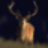
\includegraphics[width=\frameSize cm,height=\frameSize cm]{CIFAR10_example}};
\end{scope}

% The side thickness (yz plane)
% Stays at x=0 (left side), but height must match frameSize
\begin{scope}[canvas is yz plane at x=0]
\draw[fill=gray!50, draw=gray!50] (0, \i*\frameDist) rectangle (\frameSize, \i*\frameDist - \frameThick);
\end{scope}
    
% The top thickness (xz plane)
% Move the plane from 'y=2' to 'y=\frameSize'
\begin{scope}[canvas is xz plane at y=\frameSize] 
\draw[fill=gray!20, draw=gray!20] (0, \i*\frameDist) rectangle (\frameSize, \i*\frameDist - \frameThick);
\end{scope}
} % End of foreach loop

% 3D Scope (left)
\end{scope}



% 2D scope
\begin{scope}[reset cm, x={(1cm,0cm)}, y={(0cm,1cm)}]

% Left arrow
\coordinate (arrowLeft) at ({\arrowDist * (\frameSize + \frameDist )}, {0.75*\frameSize});
\coordinate (arrowRight) at ($(arrowLeft) + (\arrowLength, 0)$);
\draw[-latex, ultra thick] (arrowLeft) -- (arrowRight);

% Spike Plot
% Plot axes corners
\coordinate (plotOrigin) at ($(arrowRight)+(\plotDist, -\plotSize*0.5)$);
\coordinate (plotY) at ($(arrowRight)+(\plotDist, \plotSize*0.5)$);
\coordinate (plotX) at ($(arrowRight)+(\plotDist + \plotSize, -\plotSize*0.5)$);
% Plot axes ->
\draw[-latex, thick] (plotOrigin) -- (plotX);
\draw[-latex, thick] (plotOrigin) -- (plotY);

% Input and plot nodes
\node[below] at ($(plotX)$) {\textbf{T}};
\node[above, align=center] at ($(plotY) + (0.45*\plotSize, 0)$) {\textbf{Input Spike Trains}};
\node[above, align=center] at ($(plotY) + (-3, 0)$) {\textbf{Input CIFAR10 Samples}};

\foreach \i in {0, 1, 2, 3} {
% Plot grid lines
\draw ($(plotOrigin)+(0, \i*0.25*\plotSize)$) -- ($(plotX)+(-\plotBorder, \i*0.25*\plotSize)$);
\draw[dashed] ($(plotOrigin)+(\i*0.2*\plotSize, 0) + (0.2*\plotSize, 0)+(-\plotBorder*0.5, 0)$) -- ($(plotY)+(\i*0.2*\plotSize, -\plotBorder)+(0.2*\plotSize, 0)+(-\plotBorder*0.5, 0)$);

% Plot spikes from arrays
% Get the value of all spike arrays for current \i
\pgfmathparse{\rowAspikes[\i]}
\let\rowA\pgfmathresult
\pgfmathparse{\rowBspikes[\i]}
\let\rowB\pgfmathresult
\pgfmathparse{\rowCspikes[\i]}
\let\rowC\pgfmathresult
\pgfmathparse{\rowDspikes[\i]}
\let\rowD\pgfmathresult

% Get position for bottom left spike (other spikes can be adapted from it)
\coordinate (spikeDef) at ($(plotOrigin)+(0.1*\plotSize, 0)+(-\plotBorder*0.5, 0)$);

% Draw spike for populated positions
\ifnum\rowA=1
\draw[draw=red, fill=orange] ($(spikeDef)+(-\spikeWidth, 0)+(0.2*\plotSize*\i, 0)$) rectangle ($(spikeDef)+(\spikeWidth, \spikeHeight) + (0.2*\plotSize*\i, 0)$);
\fi
\ifnum\rowB=1
\draw[draw=red, fill=orange] ($(spikeDef)+(-\spikeWidth, 0.25*\plotSize)+(0.2*\plotSize*\i, 0)$) rectangle ($(spikeDef)+(\spikeWidth, \spikeHeight) + (0.2*\plotSize*\i, 0.25*\plotSize)$);
\fi
\ifnum\rowC=1
\draw[draw=red, fill=orange] ($(spikeDef)+(-\spikeWidth, 0.5*\plotSize)+(0.2*\plotSize*\i, 0)$) rectangle ($(spikeDef)+(\spikeWidth, \spikeHeight) + (0.2*\plotSize*\i, 0.5*\plotSize)$);
\fi
\ifnum\rowD=1
\draw[draw=red, fill=orange] ($(spikeDef)+(-\spikeWidth, 0.75*\plotSize)+(0.2*\plotSize*\i, 0)$) rectangle ($(spikeDef)+(\spikeWidth, \spikeHeight) + (0.2*\plotSize*\i, 0.75*\plotSize)$);
\fi
}

% Right arrow
\coordinate (RarrowLeft) at ($(arrowRight)+(2*\plotDist,0)+(\plotSize,0)$);
\coordinate (RarrowRight) at ($(RarrowLeft) + (\RarrowLength, 0)$);
\draw[-latex, ultra thick] (RarrowLeft) -- (RarrowRight);

% Top and bottom arrow
\draw[-latex, ultra thick, rounded corners=\frameRadius] ($(RarrowLeft)!0.3!(RarrowRight)$) -- 
($(RarrowLeft)!0.3!(RarrowRight) + (0, \vertDist)$) --
($(RarrowRight) + (0, \vertDist)$);
\draw[-latex, ultra thick, rounded corners=\frameRadius] ($(RarrowLeft)!0.3!(RarrowRight)$) -- 
($(RarrowLeft)!0.3!(RarrowRight) + (0, -\vertDist)$) --
($(RarrowRight) + (0, -\vertDist)$);

% Q K V Labels
\draw[above] node at ($(RarrowLeft)!0.8!(RarrowRight)$) {\textbf{K}};
\draw[above] node at ($(RarrowLeft)!0.8!(RarrowRight) + (0, \vertDist)$) {\textbf{Q}};
\draw[above] node at ($(RarrowLeft)!0.8!(RarrowRight) + (0, -\vertDist)$) {\textbf{V}};


% 2D scope
\end{scope}


% 2D scope (right)
\begin{scope}[shift={($(RarrowRight)+(0.75*\RarrowDist,0)$)}]

% Foreach column left to right
\foreach \i in {0, 1, 2, 3, 4, 5} {

% Get the horizontal offset of the column
\pgfmathsetmacro{\horOff}{\i*\vertDist + 2*\groupDist}
\ifnum\i<4
\pgfmathsetmacro{\horOff}{\i*\vertDist + \groupDist}
\fi
\ifnum\i<2
\pgfmathsetmacro{\horOff}{\i*\vertDist}
\fi

% 2D scope ofset to column
\begin{scope}[shift={(\horOff, 0)}]
% Foreach row from bottom to top
\foreach \j in {-2, -1, 0, 1} {
% 2D scope ofset to row
\begin{scope}[shift={(0, \j*\vertDist)}]

% This scope will occur once per attension in the 4x3 region, centered in the square center

% Check if this is row -2 and in avg row
\pgfmathparse{(\j != -2) || and(\i != 2, \i != 3) ? 1 : 0} \ifnum\pgfmathresult=1

% Get offset for average blocks
\pgfmathsetmacro{\avgVert}{0.0}
\ifnum\j=-2
\pgfmathsetmacro{\avgVert}{0.5}
\fi

% Get square coordinates for current gird position
\pgfmathsetmacro{\offset}{0.5*(\vertDist - \vertBorder)}
\coordinate (bottomLeft) at ({-\offset, -\offset - \avgVert});
\coordinate (bottomRight) at ({\offset, -\offset - \avgVert});
\coordinate (topLeft) at ({-\offset, \offset - \avgVert});
\coordinate (topRight) at ({\offset, \offset - \avgVert});
\draw (bottomLeft) rectangle (topRight);
% Get dim distance (square face / dim)
\pgfmathsetmacro{\dimSize}{(\vertDist - \vertBorder) / \attDim}


% Fill all square faces with their colors and background banners
\ifnum\j=-2
\fill[avgColor!20!white, rounded corners=\frameRadius] 
($(topLeft)+(-0.5*\frameBorder,0.5*\frameBorder)$) rectangle
($(bottomRight)+({0.5*\frameBorder+\dimSize},-0.5*\frameBorder)$);
\fill[avgColor] (bottomLeft) rectangle (topRight);
\fill[avgColor!80!black] (topLeft) -- 
($(topLeft)+(0.781*\dimSize, 0.625*\dimSize)$) -- 
($(topRight)+(0.781*\dimSize, 0.625*\dimSize)$) -- (topRight) -- cycle;
\fill[avgColor!60!black] (topRight) -- 
($(topRight)+(0.781*\dimSize, 0.625*\dimSize)$) -- 
($(bottomRight)+(0.781*\dimSize, 0.625*\dimSize)$) -- (bottomRight) -- cycle;
\fi
\ifnum\j=-1
\fill[botColor!20!white, rounded corners=\frameRadius] 
($(topLeft)+(-0.5*\frameBorder,0.5*\frameBorder)$) rectangle
($(bottomRight)+({0.5*\frameBorder+\dimSize},-0.5*\frameBorder)$);
\fill[botColor] (bottomLeft) rectangle (topRight);
\fill[botColor!80!black] (topLeft) -- 
($(topLeft)+(0.781*\dimSize, 0.625*\dimSize)$) -- 
($(topRight)+(0.781*\dimSize, 0.625*\dimSize)$) -- (topRight) -- cycle;
\fill[botColor!60!black] (topRight) -- 
($(topRight)+(0.781*\dimSize, 0.625*\dimSize)$) -- 
($(bottomRight)+(0.781*\dimSize, 0.625*\dimSize)$) -- (bottomRight) -- cycle;
\fi
\ifnum\j=0
\fill[midColor!20!white, rounded corners=\frameRadius] 
($(topLeft)+(-0.5*\frameBorder,0.5*\frameBorder)$) rectangle
($(bottomRight)+({0.5*\frameBorder+\dimSize},-0.5*\frameBorder)$);
\fill[midColor] (bottomLeft) rectangle (topRight);
\fill[midColor!80!black] (topLeft) -- 
($(topLeft)+(0.781*\dimSize, 0.625*\dimSize)$) -- 
($(topRight)+(0.781*\dimSize, 0.625*\dimSize)$) -- (topRight) -- cycle;
\fill[midColor!60!black] (topRight) -- 
($(topRight)+(0.781*\dimSize, 0.625*\dimSize)$) -- 
($(bottomRight)+(0.781*\dimSize, 0.625*\dimSize)$) -- (bottomRight) -- cycle;
\fi
\ifnum\j=1
\fill[topColor!20!white, rounded corners=\frameRadius] 
($(topLeft)+(-0.5*\frameBorder,0.5*\frameBorder)$) rectangle
($(bottomRight)+({0.5*\frameBorder+\dimSize},-0.5*\frameBorder)$);
\fill[topColor] (bottomLeft) rectangle (topRight);
\fill[topColor!80!black] (topLeft) -- 
($(topLeft)+(0.781*\dimSize, 0.625*\dimSize)$) -- 
($(topRight)+(0.781*\dimSize, 0.625*\dimSize)$) -- (topRight) -- cycle;
\fill[topColor!60!black] (topRight) -- 
($(topRight)+(0.781*\dimSize, 0.625*\dimSize)$) -- 
($(bottomRight)+(0.781*\dimSize, 0.625*\dimSize)$) -- (bottomRight) -- cycle;
\fi


% Draw DxD faces
\draw (bottomLeft) rectangle (topRight);

% Draw small faces on each front face
\foreach \k in {1,...,\attDim} {
\draw ($(bottomLeft)+(0,\k*\dimSize)$) -- ($(bottomRight)+(0,\k*\dimSize)$);
\draw ($(bottomLeft)+(\k*\dimSize,0)$) -- ($(topLeft)+(\k*\dimSize,0)$);
}

% To match the angle of the other 3D section:
%36.88 degree angle
% x = 0.781
% 7 = 0.625
% For a hypotenuse of 1

% Draw side dividing lines
\foreach \k in {0,...,\attDim} {
\draw ($(topLeft)+(\k*\dimSize, 0)$) -- ($(topLeft)+(\k*\dimSize, 0)+(0.781*\dimSize, 0.625*\dimSize)$);
\draw ($(bottomRight)+(0,\k*\dimSize)$) -- 
($(bottomRight)+(0,\k*\dimSize)+(0.781*\dimSize, 0.625*\dimSize)$);
}

% Draw bounding edges
\draw ($(topLeft)+(0.781*\dimSize, 0.625*\dimSize)$) -- ($(topRight)+(0.781*\dimSize, 0.625*\dimSize)$);
\draw ($(bottomRight)+(0.781*\dimSize, 0.625*\dimSize)$) -- 
($(topRight)+(0.781*\dimSize, 0.625*\dimSize)$);

% Check if this is row -2 and in avg row
\fi

% 2D scope ofset to row
\end{scope}}
% 2D scope ofset to column
\end{scope}}


% Get coords for frames and arrows
\pgfmathsetmacro{\offset}{0.5*(\vertDist - \vertBorder)}
\coordinate (bottomLeft) at ($(-\frameBorder,-3*\offset)+(0,-0.75*\vertBorder)$);
\coordinate (topRight) at ($(2*\offset,3*\offset)+(1.4*\vertBorder,0.75*\vertBorder) + (\frameBorder, 0)$);
\pgfmathsetmacro{\dimSize}{(\vertDist - \vertBorder) / \attDim}
\pgfmathsetmacro{\dimVert}{\dimSize * 0.625}

% Draw frames
\draw[thick, rounded corners=\frameRadius]
($(bottomLeft)+(-\frameBorder,-\frameBorder)$) rectangle
($(topRight)+(\frameBorder,\frameBorder)$);
\draw[thick, rounded corners=\frameRadius]
($(bottomLeft)+(-\frameBorder,-\frameBorder)+({2*\vertDist + \groupDist}, 0)$) rectangle
($(topRight)+(\frameBorder,\frameBorder)+({2*\vertDist + \groupDist}, 0)$);
\draw[thick, rounded corners=\frameRadius]
($(bottomLeft)+(-\frameBorder,-\frameBorder)+({4*\vertDist + 2*\groupDist}, 0)$) rectangle
($(topRight)+(\frameBorder,\frameBorder)+({4*\vertDist + 2*\groupDist}, 0)$);


% Draw arrows
% Top Arrows Straight
\draw[-latex, very thick] ($(0,\offset)+(0,\vertBorder)$) -- 
($(0,\offset)+(0,0.5*\dimVert)$);
\draw[-latex, very thick] ($(\vertDist,\offset)+(0,\vertBorder)$) -- 
($(\vertDist,\offset)+(0,0.5*\dimVert)$);
\draw[-latex, very thick] ($({2*\vertDist+\groupDist},\offset)+(0,\vertBorder)$) -- 
($({2*\vertDist+\groupDist},\offset)+(0,0.5*\dimVert)$);
\draw[-latex, very thick] ($({3*\vertDist+\groupDist},\offset)+(0,\vertBorder)$) -- 
($({3*\vertDist+\groupDist},\offset)+(0,0.5*\dimVert)$);
\draw[-latex, very thick] ($({4*\vertDist+2*\groupDist},\offset)+(0,\vertBorder)$) -- 
($({4*\vertDist+2*\groupDist},\offset)+(0,0.5*\dimVert)$);
\draw[-latex, very thick] ($({5*\vertDist+2*\groupDist},\offset)+(0,\vertBorder)$) -- 
($({5*\vertDist+2*\groupDist},\offset)+(0,0.5*\dimVert)$);

% Bottom Arrows Straight
\draw[-latex, very thick] ($(0,-2*\offset)+(0,\vertBorder)$) -- 
($(0,-2*\offset)+(0,0.5*\dimVert)$);
\draw[-latex, very thick] ($(\vertDist,-2*\offset)+(0,\vertBorder)$) -- 
($(\vertDist,-2*\offset)+(0,0.5*\dimVert)$);
\draw[-latex, very thick] ($({2*\vertDist+\groupDist},-2*\offset)+(0,\vertBorder)$) -- 
($({2*\vertDist+\groupDist},-2*\offset)+(0,0.5*\dimVert)$);
\draw[-latex, very thick] ($({3*\vertDist+\groupDist},-2*\offset)+(0,\vertBorder)$) -- 
($({3*\vertDist+\groupDist},-2*\offset)+(0,0.5*\dimVert)$);
\draw[-latex, very thick] ($({4*\vertDist+2*\groupDist},-2*\offset)+(0,\vertBorder)$) -- 
($({4*\vertDist+2*\groupDist},-2*\offset)+(0,0.5*\dimVert)$);
\draw[-latex, very thick] ($({5*\vertDist+2*\groupDist},-2*\offset)+(0,\vertBorder)$) -- 
($({5*\vertDist+2*\groupDist},-2*\offset)+(0,0.5*\dimVert)$);

% Average Arrows Straight
\draw[-latex, very thick] ($(0,-5*\offset)+(0,\vertBorder)$) -- 
($(0,-5.75*\offset)+(0,0.5*\dimVert)$);
\draw[-latex, very thick] ($(\vertDist,-5*\offset)+(0,\vertBorder)$) -- 
($(\vertDist,-5.75*\offset)+(0,0.5*\dimVert)$);
\draw[-latex, very thick] ($({4*\vertDist+2*\groupDist},-5*\offset)+(0,\vertBorder)$) -- 
($({4*\vertDist+2*\groupDist},-5.75*\offset)+(0,0.5*\dimVert)$);
\draw[-latex, very thick] ($({5*\vertDist+2*\groupDist},-5*\offset)+(0,\vertBorder)$) -- 
($({5*\vertDist+2*\groupDist},-5.75*\offset)+(0,0.5*\dimVert)$);

% Average Diagonal
\draw[-latex, very thick] ($({2*\vertDist+\groupDist},-5.05*\offset)+(0,\vertBorder)$) -- 
($(\vertDist,-5.75*\offset)+(0,0.5*\dimVert)$);
\draw[-latex, very thick] ($({3*\vertDist+\groupDist},-5.05*\offset)+(0,\vertBorder)$) -- 
($({4*\vertDist+2*\groupDist},-5.75*\offset)+(0,0.5*\dimVert)$);

% Top Arrows Diagonal
\draw[-latex, very thick] ($(0,\offset)+(0,\vertBorder)$) -- 
($(\vertDist,\offset)+(0,0.5*\dimVert)$);
\draw[-latex, very thick] ($(\vertDist,\offset)+(0,\vertBorder)$) -- 
($(0,\offset)+(0,0.5*\dimVert)$);
\draw[-latex, very thick] ($({2*\vertDist+\groupDist},\offset)+(0,\vertBorder)$) -- 
($({3*\vertDist+\groupDist},\offset)+(0,0.5*\dimVert)$);
\draw[-latex, very thick] ($({3*\vertDist+\groupDist},\offset)+(0,\vertBorder)$) -- 
($({2*\vertDist+\groupDist},\offset)+(0,0.5*\dimVert)$);
\draw[-latex, very thick] ($({4*\vertDist+2*\groupDist},\offset)+(0,\vertBorder)$) -- 
($({5*\vertDist+2*\groupDist},\offset)+(0,0.5*\dimVert)$);
\draw[-latex, very thick] ($({5*\vertDist+2*\groupDist},\offset)+(0,\vertBorder)$) -- 
($({4*\vertDist+2*\groupDist},\offset)+(0,0.5*\dimVert)$);

% Bottom Arrows Diagonal
\draw[-latex, very thick] ($(0,-2*\offset)+(0,\vertBorder)$) -- 
($(\vertDist,-2*\offset)+(0,0.5*\dimVert)$);
\draw[-latex, very thick] ($(\vertDist,-2*\offset)+(0,\vertBorder)$) -- 
($(0,-2*\offset)+(0,0.5*\dimVert)$);
\draw[-latex, very thick] ($({2*\vertDist+\groupDist},-2*\offset)+(0,\vertBorder)$) -- 
($({3*\vertDist+\groupDist},-2*\offset)+(0,0.5*\dimVert)$);
\draw[-latex, very thick] ($({3*\vertDist+\groupDist},-2*\offset)+(0,\vertBorder)$) -- 
($({2*\vertDist+\groupDist},-2*\offset)+(0,0.5*\dimVert)$);
\draw[-latex, very thick] ($({4*\vertDist+2*\groupDist},-2*\offset)+(0,\vertBorder)$) -- 
($({5*\vertDist+2*\groupDist},-2*\offset)+(0,0.5*\dimVert)$);
\draw[-latex, very thick] ($({5*\vertDist+2*\groupDist},-2*\offset)+(0,\vertBorder)$) -- 
($({4*\vertDist+2*\groupDist},-2*\offset)+(0,0.5*\dimVert)$);

% Time t labels
\node[] (t1) at ($(0,5*\offset)+(0,0.5*\dimVert)$) {\textbf{T=1}};
\node[] (t2) at ($(\vertDist,5*\offset)+(0,0.5*\dimVert)$) {\textbf{T=2}};
\node[] (t3) at ($({2*\vertDist+\groupDist},5*\offset)+(0,0.5*\dimVert)$) {\textbf{T=2}};
\node[] (t4) at ($({3*\vertDist+\groupDist},5*\offset)+(0,0.5*\dimVert)$) {\textbf{T=3}};
\node[] (t5) at ($({4*\vertDist+2*\groupDist},5*\offset)+(0,0.5*\dimVert)$) {\textbf{T=3}};
\node[] (t6) at ($({5*\vertDist+2*\groupDist},5*\offset)+(0,0.5*\dimVert)$) {\textbf{T=4}};

% Block labels
\node [] at ($(t1)!0.5!(t2) + (0, 0.5)$) {\textbf{Block 1}};
\node [] at ($(t3)!0.5!(t4) + (0, 0.5)$) {\textbf{Block 2}};
\node [] at ($(t5)!0.5!(t6) + (0, 0.5)$) {\textbf{Block 3}};

% Time t average labels
\node[align=center] (at1) at ($(0,-8.75*\offset)+(0,0.5*\dimVert)$) {\textbf{T=1}};
\node[align=center] (at2) at ($(\vertDist,-8.75*\offset)+(0,0.5*\dimVert)$) {\textbf{T=2}};
\node[align=center] (at3) at ($({4*\vertDist+2*\groupDist},-8.75*\offset)+(0,0.5*\dimVert)$) {\textbf{T=3}};
\node[align=center] (at4) at ($({5*\vertDist+2*\groupDist},-8.75*\offset)+(0,0.5*\dimVert)$) {\textbf{T=4}};

% Average labels
\node [] at ($(at1)!0.5!(at2) + (0, -0.5)$) {\textbf{Average}};
\node [] at ($(at3)!0.5!(at4) + (0, -0.5)$) {\textbf{Average}};

% 2D scope (right)
\end{scope}

\end{tikzpicture}}
\end{document}